\section{The Running Example: Automatic Sliding Door}
\label{sec:example}
Our running example for this demo is a sliding door system of PLC based
controller. The controller for this system is shown in fig~\ref{fig:sliding_doors_example}. The shown controller implements the
following behavior,
\begin{itemize}
  \item the sliding door opens if somebody enters by sensing the object using
  the infrared sensor (X0),
  \item the sliding door opens until the opening limits are reached, also
  detected by the sensor (X2),
  \item upon reaching the opening limits the count down timer starts and
  \item closes the door when the timer expires until the closing limit is
  reached detected by (X1).
\end{itemize}
\begin{figure*}[!h]
\centering
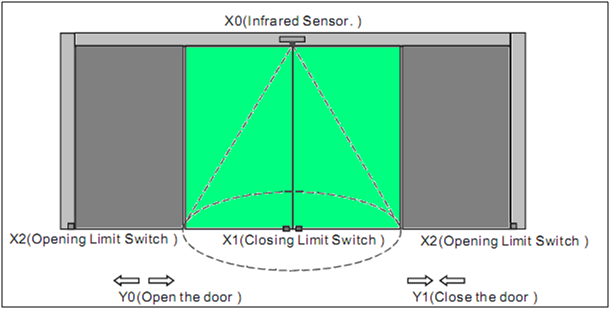
\includegraphics[width=1\textwidth]{./images/SlidingDoors.png}
\caption{A running example of Sliding Doors}
\label{fig:sliding_doors_example}
\end{figure*}